%%%%%%%%%%%%%%%%%%%%%%%%%%%%%%%%%%%%%%%%%
% Beamer Presentation
% LaTeX Template
% Version 1.0 (10/11/12)
%
% This template has been downloaded from:
% http://www.LaTeXTemplates.com
%
% License:
% CC BY-NC-SA 3.0 (http://creativecommons.org/licenses/by-nc-sa/3.0/)
%
%%%%%%%%%%%%%%%%%%%%%%%%%%%%%%%%%%%%%%%%%

%----------------------------------------------------------------------------------------
%	PACKAGES AND THEMES
%----------------------------------------------------------------------------------------

\documentclass[10pt]{beamer}

\mode<presentation> {

% The Beamer class comes with a number of default slide themes
% which change the colors and layouts of slides. Below this is a list
% of all the themes, uncomment each in turn to see what they look like.

%\usetheme{default}
%\usetheme{AnnArbor}
%\usetheme{Antibes}
%\usetheme{Bergen}
%\usetheme{Berkeley}
%\usetheme{Berlin}
%\usetheme{Boadilla}
%\usetheme{CambridgeUS}
%\usetheme{Copenhagen}
%\usetheme{Darmstadt}
%\usetheme{Dresden}
%\usetheme{Frankfurt}
%\usetheme{Goettingen}
%\usetheme{Hannover}
%\usetheme{Ilmenau}
%\usetheme{JuanLesPins}
%\usetheme{Luebeck}
\usetheme{Madrid}
%\usetheme{Malmoe}
%\usetheme{Marburg}
%\usetheme{Montpellier}
%\usetheme{PaloAlto}
%\usetheme{Pittsburgh}
%\usetheme{Rochester}
%\usetheme{Singapore}
%\usetheme{Szeged}
%\usetheme{Warsaw}

% As well as themes, the Beamer class has a number of color themes
% for any slide theme. Uncomment each of these in turn to see how it
% changes the colors of your current slide theme.

%\usecolortheme{albatross}
%\usecolortheme{beaver}
%\usecolortheme{beetle}
%\usecolortheme{crane}
%\usecolortheme{dolphin}
%\usecolortheme{dove}
%\usecolortheme{fly}
%\usecolortheme{lily}
%\usecolortheme{orchid}
%\usecolortheme{rose}
%\usecolortheme{seagull}
%\usecolortheme{seahorse}
%\usecolortheme{whale}
%\usecolortheme{wolverine}

%\setbeamertemplate{footline} % To remove the footer line in all slides uncomment this line
%\setbeamertemplate{footline}[page number] % To replace the footer line in all slides with a simple slide count uncomment this line

%\setbeamertemplate{navigation symbols}{} % To remove the navigation symbols from the bottom of all slides uncomment this line
}

\usepackage{graphicx} % Allows including images
\usepackage{booktabs} % Allows the use of \toprule, \midrule and \bottomrule in tables
%\usepackage{hyperref}
%\usepackage{footnote}
%\usepackage{tikz}
\usepackage{adjustbox} 

%----------------------------------------------------------------------------------------
%	TITLE PAGE
%----------------------------------------------------------------------------------------

\title[]{Retail Traders Through Booms and Busts} % The short title appears at the bottom of every slide, the full title is only on the title page
\subtitle{Evidence from Robinhood}

\author{Pietro Reggiani} % Your name
\institute[] % Your institution as it will appear on the bottom of every slide, may be shorthand to save space
{PhD Second Year Paper Presentation}
\date{\today} % Date, can be changed to a custom date


\begin{document}

\begin{frame}
\titlepage % Print the title page as the first slide
\end{frame}


%----------------------------------------------------------------------------------------
%	PRESENTATION SLIDES
%----------------------------------------------------------------------------------------

 
\begin{frame}{Introduction}

The focus is on:
\begin{itemize}[<+->]
\item Investor Behaviour 
\item Retail Investors
\item Peculiar Young sub-sample
\item Investment choices during booms and busts
\end{itemize}

\pause

\vspace{5mm}
This exercise:
\begin{itemize}[<+->]
\item Data from Popular trading app \textit{Robinhood}
\item Describe Cross-Section of Stock Popularity
\item Covid Shock provides bust and boom
\item Which stock characteristics matter for retail investors ?
\end{itemize}

\end{frame}


\begin{frame}{Retail Investors Pandemic Frenzy}

\begin{itemize}
\item Zero-commission trading platforms boom since Covid outbreak \pause
\includegraphics<2>[scale=0.2]{../../material/news_articles/cnbc_title.PNG} 
\pause
\vspace{7mm}
\item Worries over excessive speculation \pause \vspace{3mm}

\begin{center}

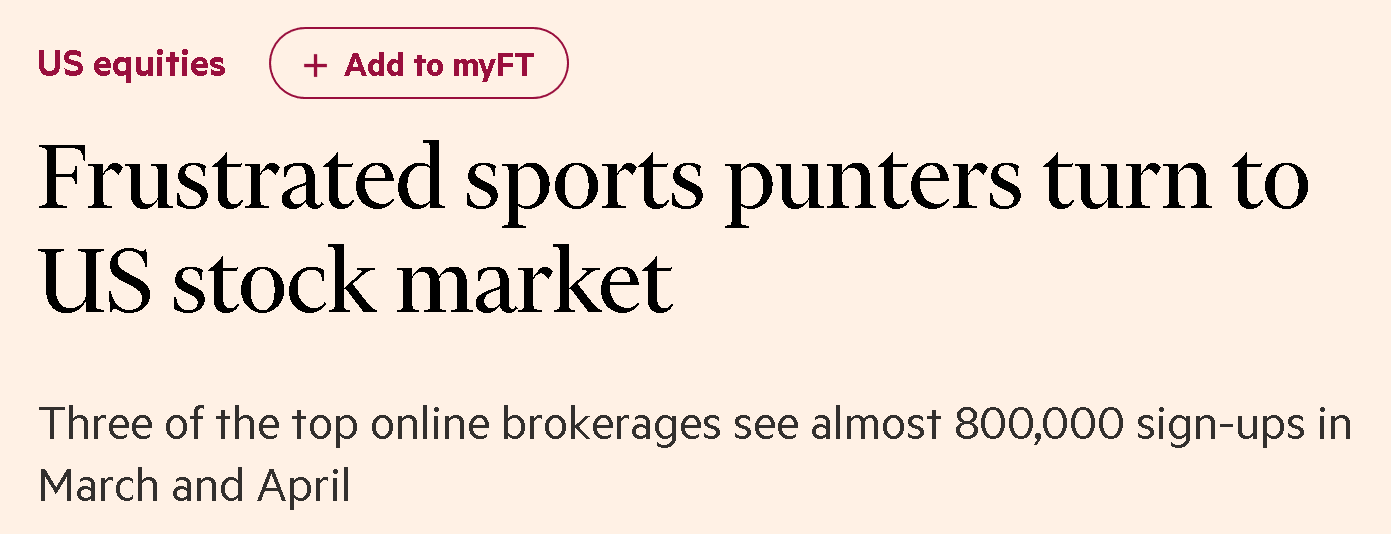
\includegraphics[scale=0.2]{../../material/news_articles/FT_robinhood_frustrated_gamblers_title.PNG}<4-5> \vspace{2mm}
\pause

\only<5>{
\begin{quote}
``A casino or stock market? Retail buying frenzy goes wild."\\
 \tiny{(Thomson Reuters Jun 10th)}
\end{quote} 
}
\end{center}
\pause

\item and on bankrupt firm bets

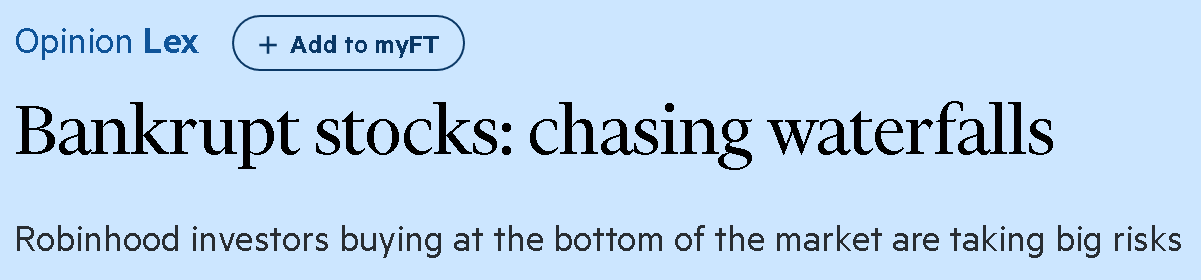
\includegraphics[scale=0.3]{../../material/news_articles/FT_robinhood_bankrupt_stocks_title.PNG} 


\end{itemize}

\end{frame}

\begin{frame}{Related Literature \& Contribution}
About Retail Investors, we know: \pause
\begin{itemize}[<+->]
\item Some of their behavioural patterns \\ (Barber and Odean 2013 for a review)
\item How their beliefs affect choices (Giglio Stroebel et al. 2020)
\item Their Expectations dynamics during Covid pandemic  \\ (Giglio, Stroebel et al. 2020$^2$)
\item Prone to gamble on "lottery stocks" \\ (Han\& Kumar 2013, Coelho et al. 2014)
\end{itemize}

\pause
today:
\begin{itemize}[<+->]
\item Focus on Peculiar Young \textit{Robinhood} sample
\item Describe Cross-Section of Stock Popularity Pre-Pandemic 
\item Exploit Covid Collapse \& Recovery to observe reaction
\item Which stocks gained popularity in market collapse?
\item And in the recent recovery?
\end{itemize}

\end{frame}



\begin{frame}{Robinhood Data}
\only<1>{
The platform\footnote{\tiny  https://www.businessofapps.com/data/robinhood-statistics/}:
\begin{itemize}
\item Founded in 2015, 73\% of tot. Historical Revenues in 2020H1
\item 13 Million users
\item Popular among Millennials (avg. age 31) 
\item Avg. Account size 1-5\$k
\item Total AUM ca. \$20bn
\end{itemize} } \pause

\only<2-6> { The Data:
\begin{itemize}
\item Stocks \& ADRs listed in U.S. exchanges (no funds nor derivatives) \pause
\item \textbf<3-5>{Number} of users holding each stock - Daily \pause
\item Do not know value of holding \pause
\item Do not know total number of users on the platform \pause
\item $\Rightarrow$ Focus on \textbf{Number of Users at Stock Level} 
\end{itemize} }
\pause
\only<7>{
\begin{figure}[h!]
\centering
\includegraphics[scale=0.45]{../../output/charts/value.png}
\end{figure} }

\pause

\only<3>{\vspace{10mm} $\Rightarrow$ Focus on Number of Users at  \textbf{firm level}}
\end{frame}

\begin{frame}{Other Data and Sample Selection}
merge to:
\begin{itemize}
\item Daily prices from \textit{Compustat North America} 
\item Accounting Variables from \textit{Compustat Fundamentals Annual }
\item ESG scores from \textit{Thomson Reuters Asset4}
\item Market return from \textit{Ken French}
\end{itemize}
\pause \vspace{5mm}
choices:
\begin{itemize}
\item Only Stocks Ordinary Common Shares and ADRs 
\item Only NYSE, AMEX and Nasdaq
\item Exclude Financial Firms (GICS 40)
\end{itemize}
\pause \vspace{5mm}
final sample:
\begin{itemize}
\item Panel $\approx$3'700 stock-users, daily May2018-Aug2020
\end{itemize}

\end{frame}

\begin{frame}{Cross Section of Popularity Pre-Pandemic}
\only<1>{
\begin{itemize}
\item Which characteristics explain stock popularity?
\item Daily Firm-Level Users May 2018 to Feb 21st 2020
\end{itemize}  }

\only<2>{ \vspace{-3mm} \centering
\scalebox{0.75}{
\small
\input{../../output/tables/pre_fe_tab_enscore_slides}
}
}

\end{frame}

\begin{frame}{Reactions to Pandemic Shock}
\begin{itemize}[<+->]
\item S\&P500 collapsed by a third from Feb 20th to March 20th
\item Then rebounded vigorously... \vspace{5mm}
\item how do investors react?
\item which characteristics predict flow of investors?
\item is crash different from recovery?
\end{itemize}
\end{frame}

\begin{frame}{Examples of Pandemic Popularity Winners}

\only<1-4>{

Some stocks boomed since the crash...  \vspace{5mm}

\only<2>{ \centering
\includegraphics[scale=0.5]{../../output/charts/AMZN.png} 
}
 \only<3>{ \centering
\includegraphics[scale=0.5]{../../output/charts/TSLA.png} 
}
\only<4>{ \centering
\includegraphics[scale=0.5]{../../output/charts/MRNA.png} 
}

}

\only<5-6>{

Some other solid ones did well  \vspace{5mm}

\only<6>{ \centering
\includegraphics[scale=0.5]{../../output/charts/MSFT.png} 
}
}

\only<7->{

While others crashed... \only<8->{?!}  \vspace{5mm}

\only<8>{ \centering
\includegraphics[scale=0.5]{../../output/charts/AAL.png} 
}

\only<9>{ \centering
\includegraphics[scale=0.5]{../../output/charts/CCL.png} 
}

\only<10>{ \centering
\includegraphics[scale=0.5]{../../output/charts/HTZ.png} 
}


}

\end{frame}

\begin{frame}{Industry Popularity In Pandemic}

\only<1>{ \centering
\includegraphics[scale=0.55]{../../output/charts/sectors_crash.png} 
}

\only<2>{ \centering
\includegraphics[scale=0.55]{../../output/charts/sectors_recovery.png} 
}

\end{frame}



\begin{frame}{Changes in Users}

\begin{itemize}[<+->]
\item Does not exactly look like a flight to quality
\item Can Stock characteristics explain popularity evolution?
\end{itemize}


\end{frame}


\begin{frame}{Cross-section of Popularity Changes - Crash}

\only<1>{
$$  \log(users_{g,i,t+1})- \log(users_{g,i,t})  = \alpha \log(users_{g,i,t}) + \beta \mathbf{x_{i,t}} + \gamma_g + \varepsilon_{i,t} $$
\vspace{7mm}
\begin{itemize}
\item $t=$ Fri \textbf{Feb 21st} , $(t+1)=$ Fri \textbf{Mar 20th} \vspace{2mm}
\item Firm $i$, within industry $g$ \vspace{2mm}
\item $\mathbf{x_{i,t}}$ firm characteristics as of time $t$ \vspace{2mm}
\item Accounting Variables as of EoY 2019
\end{itemize}

}

\pause

\centering  \vspace{-3mm}
\scalebox{0.71}{
\small
\input{../../output/tables/crash_fe_tab_enscore_slides}
}


\end{frame}






\begin{frame}{Cross-section of Popularity Changes - Recovery}

\only<1>{
$$  \log(users_{g,i,t+1})- \log(users_{g,i,t})  = \alpha \log(users_{g,i,t}) + \beta \mathbf{x_{i,t}} + \gamma_g + \varepsilon_{i,t} $$
\vspace{7mm}
\begin{itemize}
\item $t=$ Fri \textbf{Mar 20th} , $(t+1)=$ Fri \textbf{Aug 7th} \vspace{2mm}
\item Firm $i$, within industry $g$ \vspace{2mm}
\item $\mathbf{x_{i,t}}$ firm characteristics as of time $t$ \vspace{2mm}
\item Accounting Variables as of EoY 2019
\end{itemize}

}

\pause

\centering  \vspace{-3mm}
\scalebox{0.71}{
\small
\input{../../output/tables/recovery_fe_tab_enscore_slides}
}


\end{frame}


\begin{frame}{Conclusion}

in this exercise:
\begin{itemize}[<+->]
\item peculiar new sub-sample of young retail investors
\item analysis of stock popularity through boom and bust
\item no evidence of flight to quality
\item rather of "flight to zombies"
\item no evidence of green stocks resilience
\end{itemize}
\pause \vspace{3mm}
going forward:
\begin{itemize}
\item Spreading Adoption of Trading Apps in Population
\item Important to improve understanding of household risk taking
\end{itemize}


\end{frame}







\end{document}